%!TEX root =  main.tex

\lectureheader{162}{Calculus II}{Hyperbolic functions}{\textit{Thomas' Calculus} \textsection 7.7}

\begin{definition}
We define the \textbf{hyperbolic sine} by the rule
\begin{equation*}
\sinh x = \frac{\E^x-\E^{-x}}{2} \quad (x\in\R)
\end{equation*}
and the \textbf{hyperbolic cosine} by the rule
\begin{equation*}
\cosh x = \frac{\E^x+\E^{-x}}{2} \quad (x\in\R).
\end{equation*}
\end{definition}

\begin{remark}\,
\begin{itemize}
\item These functions are affectionately referred to as ``cinch" and ``kosh."
\item The ordinary sine and cosine are sometimes called ``circular" functions because they parameterize circles.
If $t\in [0,2\pi)$, then the point $(x,y) = (\cos t, \sin t)$ lies on the circle
\begin{equation*}
x^2+y^2=1.
\end{equation*}
\item These hyperbolic analogues parameterize hyperbolas.
If $t\in (-\infty,\infty)$, then the point $(x,y)=(\cosh t, \sinh t)$ lies on the right branch of the hyperbola
\begin{equation*}
x^2-y^2=1.
\end{equation*}
\end{itemize}
\end{remark}

\begin{definition}
We define the \textbf{hyperbolic tangent} by the rule
\begin{equation*}
\tanh x = \frac{\sinh x}{\cosh x} \quad (x\in \R),
\end{equation*}
the \textbf{hyperbolic cosecant} by the rule
\begin{equation*}
\csch x = \frac{1}{\sinh x} \quad (x\ne 0),
\end{equation*}
the \textbf{hyperbolic secant} by the rule
\begin{equation*}
\sech x = \frac{1}{\cosh x} \quad (x\in\R),
\end{equation*}
and the \textbf{hyperbolic cotangent} by the rule
\begin{equation*}
\coth x = \frac{\cosh x}{\sinh x} \quad (x\ne 0).
\end{equation*}
\end{definition}

\newpage

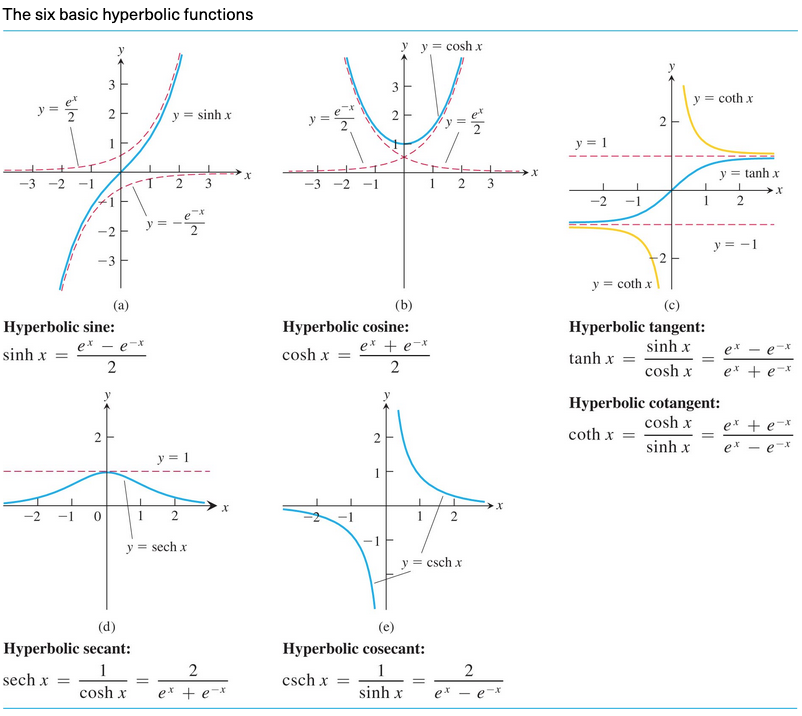
\includegraphics[width=6.5in]{img/hyperbolic_graphs}

\newpage

\begin{theorem}
For all $x$ where both sides of the identity are defined we have 
\begin{align}
\cosh^2 x -\sinh^2 x &= 1,\\
1-\tanh^2x &=\sech^2 x,\\
\coth^2 x -1&=\csch^2 x,\\
\sinh 2x &= 2\sinh x\cosh x,\\
\cosh 2x &=\cosh^2x + \sinh^2 x,\\
\cosh^2 x&=\frac{\cosh 2x + 1}{2},\\
\sinh^2 x&=\frac{\cosh 2x - 1}{2}.
\end{align}
\end{theorem}
\begin{proof}\,

\vspace{5in}
\end{proof}

\newpage

\begin{theorem}
\begin{align}
\frac{\dee}{\dee x}\sinh x &= \cosh x\quad (x\in\R)\\
\frac{\dee}{\dee x}\cosh x &= \sinh x\quad (x\in\R)\\
\frac{\dee}{\dee x}\tanh x &= \sech^2 x\quad (x\in\R)\\
\frac{\dee}{\dee x}\csch x &= -\csch x\coth x\quad (x\ne 0)\\
\frac{\dee}{\dee x}\sech x &= -\sech x\tanh x\quad (x\in \R)\\
\frac{\dee}{\dee x}\coth x &= -\csch^2 x\quad (x\ne 0)
\end{align}
\end{theorem}
\begin{remark}
Of course, each of these gives rise to a corresponding integral formula.
\end{remark}
\begin{proof}\,

\vspace{5in}
\end{proof}

\newpage

\begin{example}
Compute $\dee y/\dee x$ if $y=\tanh \sqrt{1+x^2}$.
\end{example}
\vfill

\begin{example}
Compute $\DS\int\sinh^2 x\dee x$
\end{example}
\vfill

\newpage

\begin{example}
What is the domain/range of $y=\sinh x$?
Where can we invert it?
\end{example}
\vfill

\begin{example}
What is the domain/range of $y=\cosh x$?
Where can we invert it?
\end{example}
\vfill

\newpage

\begin{definition}
The six ``inverse" hyperbolic functions are defined by the rules:
\begin{enumerate}
\item $y=\sinh^{-1} x\quad (x\in\R) \iff \sinh y = x\quad (y\in\R)$.
\item $y = \cosh^{-1} x\quad (x\ge 1) \iff \cosh y = x\quad (0\le y<\infty)$.
\item $y = \tanh^{-1} x\quad (|x|<1) \iff \tanh y = x\quad (y\in\R)$ 
\item $y=\csch^{-1} x\quad (x\ne 0)\iff \csch y = x\quad (y\ne 0)$.
\item $y = \sech^{-1} x\quad (0<x\le 1) \iff \sech y = x\quad (y\ge 0)$.
\item $y = \coth^{-1} x\quad (|x|>1) \iff \coth y = x\quad (y\ne 0)$.
\end{enumerate}
\end{definition}
\begin{remark}\,
\begin{itemize}
\item Four of these are ``true" inverses while the other two are only ``partial" inverses.
Can you figure out which?
\item We also use the notation $\arcsinh x = \sinh^{-1} x$, etc.
\end{itemize}
\end{remark}

\begin{theorem}
\begin{align}
\frac{\dee}{\dee x}\sinh^{-1} x & = \frac{1}{\sqrt{1+x^2}}\\
\frac{\dee}{\dee x}\cosh^{-1} x & = \frac{1}{\sqrt{x^2-1}}\quad (x>1)\\
\frac{\dee}{\dee x}\tanh^{-1} x & = \frac{1}{1-x^2}\quad (|x|<1)\\
\frac{\dee}{\dee x}\csch^{-1} x &=\frac{-1}{|x|\sqrt{1+x^2}}\quad (x\ne 0)\\
\frac{\dee}{\dee x}\sech^{-1} x & = \frac{-1}{x\sqrt{1-x^2}}\quad (0<x<1)\\
\frac{\dee}{\dee x}\coth^{-1} x & = \frac{1}{1-x^2}\quad (|x|>1)
\end{align}
\end{theorem}
\begin{proof}\,

\vspace{2.75in}
\end{proof}

\newpage

\begin{theorem}
\begin{align}
\int\frac{\dee x}{\sqrt{1+x^2}} &= \sinh^{-1} x + C;\\
\int\frac{\dee x}{\sqrt{x^2-1}} & = \cosh^{-1} x + C\quad (x>1);\\
\int\frac{\dee x}{1-x^2} 
&=\begin{cases}
\tanh^{-1} x + C& \text{if } |x|<1,\\
\coth^{-1} x + C& \text{if } |x|>1;
\end{cases}\\
\int\frac{\dee x}{x\sqrt{1-x^2}} &= -\sech^{-1} x + C\quad (0<x<1);\\
\int\frac{\dee x}{x\sqrt{1+x^2}} &=-\csch^{-1} |x| + C\quad (x\ne 0).
\end{align}
\end{theorem}

\begin{example}
Evaluate $\DS\int_0^1\frac{2\dee x}{\sqrt{3+4x^2}}$.
\end{example}

